% -----------------------------------------------------------
% Method
% -----------------------------------------------------------

\section{Method}


% ---------------------------------------
\subsection{Literature search}
% ---------------------------------------

Literature was searched in two rounds: first round covered all the literature until March 2018 and second round covered literature published from 2018 to October 2020. Web of Science was searched using the following terms: eye track* OR eye move* OR eye fix* AND decision making OR choice. Gray literature, such as reports and unpublished work, was identified in the first 1,000 hits on Google Scholar (200 hits in the second round). No restrictions on publication date were imposed. Additional literature was identified by searching the reference lists of the identified papers and through contact with the authors. Calls for unpublished studies were distributed to the relevant research communities via the following email lists; European Association for Decision Making (EADM), Society for Judgment and Decision Making (SJDM), and European Group of Process Tracing Studies (EGPROC). The search resulted in 412 studies screened for eligibility.


% ---------------------------------------
\subsection{Inclusion criteria}
% ---------------------------------------

We included studies in which participants made decisions or judgments between discrete alternatives while their eye movements were recorded using eye-tracking technology. We did not include studies related to perceptual judgments, such as categorizing or discriminating visual stimuli or studies on problem solving. We excluded studies where participants were selected based on clinical diagnoses or specific socio-demographic traits e.g., visual disorders, age-related visual diseases, age restrictions such as adolescents or infants. Studies using fixed exposure time or time pressure manipulations were excluded since these manipulations can influence eye movement processes \citep{orquin2018a} and lead to substantially different results \citep{simola2019a}. Included studies used either fixation likelihood (area of interest (AOI) looked at or not), fixation count (number of fixations to AOI), total dwell time (sum of durations of all fixations to an AOI), or dwell count (number of dwells to an AOI). Eventually, 69 articles met all inclusion criteria and were included in the meta-analysis (Figure~\ref{fig:flow_diagram}). Our initial literature search retrieved 2956 articles, of which 591 remained after screening of the title and abstract. Following a more detailed evaluation of whether studies were on decision making and used eye-tracking, we identified 412 articles as potentially eligible studies. Based on detailed inspection of their full texts, 69 articles satisfied all inclusion criteria and were included in the meta-analysis. Figure~\ref{fig:flow_diagram} illustrates the PRISMA flow diagram \citep{moher2009preferred}. Many of the articles consisted of multiple experiments and some experiments operationalized more than one factor. \chg{independent}{This resulted in 122 effect size estimates, out of which 50 were effects of visual factors and 72 were effects of cognitive factors}.


\begin{figure}[H]
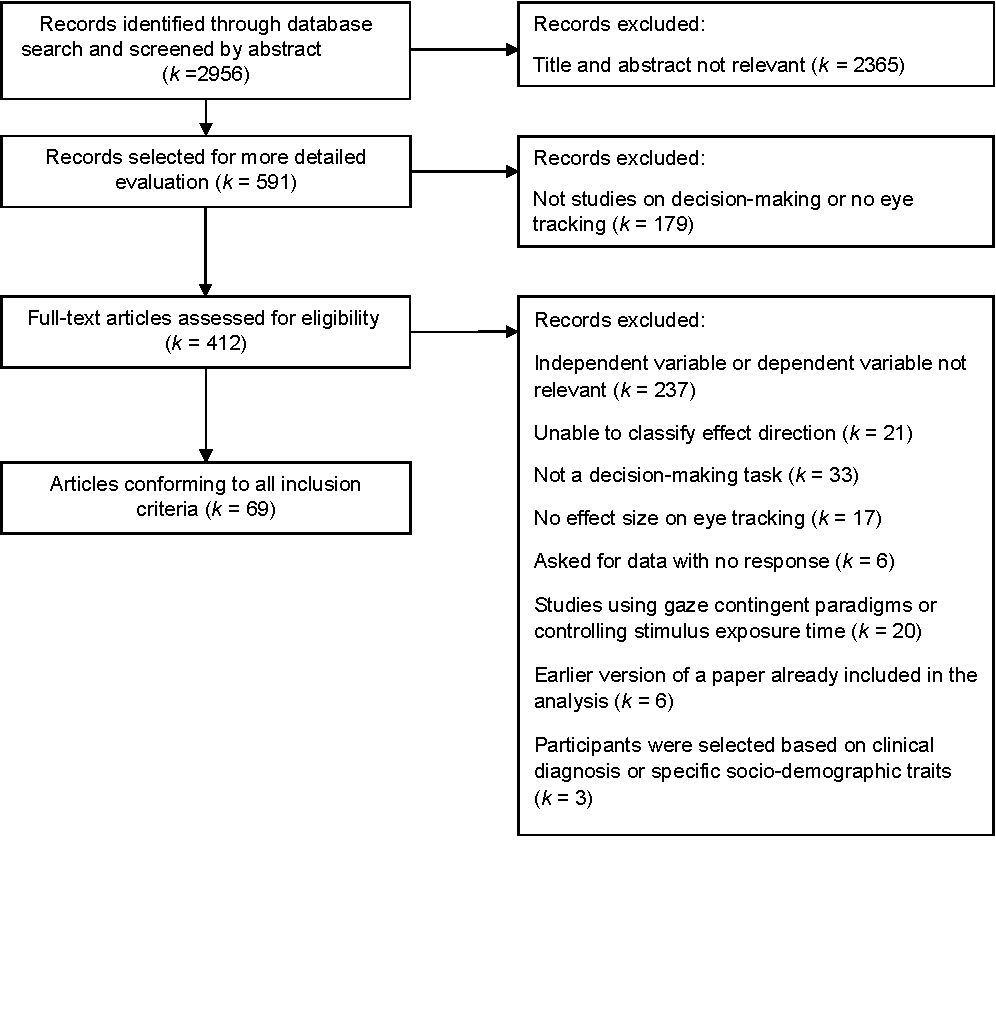
\includegraphics{prisma_update-crop}
\centering
\caption{The PRISMA flow diagram showing the results of the literature search.}
\label{fig:flow_diagram}
\end{figure}


% ---------------------------------------
\subsection{Data extraction and coding procedure}
% ---------------------------------------

The included studies were coded with regards to their (1) effect size, (2) sample size, (3) research domain, (4) eye-tracker model, (5) dependent variable, and (6) independent variable. As an additional measure we coded descriptive eye movement statistics for those studies reporting this: the mean fixation likelihood, fixation count, total dwell time, or dwell count across conditions. Although not essential to the meta-analysis, the descriptive data proved to be useful for interpreting the effect sizes. \chg{sample-information-method}{We also coded studies with regards to the participant sample characteristics including mean age, percentage of female participants, the country where the data was collected, and the ethnicity of participants. If ethnicity was not reported but country was, we coded ethnicity as the dominant ethnic group in the country where data was collected.}
Agreement for categorical variables was assessed using Cohen's kappa and for continuous variables using intraclass correlation coefficient \citep{shrout1979a}. Overall, there was a high level of agreement: effect size, $\textrm{ICC} = 0.923$, sample size, $\textrm{ICC} = 0.996$, research domain, $\textrm{ICC} = 0.731$, eye tracker model, $\textrm{ICC} = 1$, dependent variable, $\kappa = 0.923$, independent variable, $\kappa = 0.934$\unskip. While revising the manuscript, effect sizes were coded again. The revised coding of effect sizes had a high agreement with the original one,  $\textrm{ICC} = 0.923$\unskip. \chg{nonlisted-variables}{We have not explored or analyzed variables other than those described here.}

Coding of effect sizes is described in detail below, and sample size was coded as the total number of participants in a study. The research domain was coded as preferential consumer choice, inferential consumer choice, preferential non consumer choice, inferential non-consumer choice, and risky gambles. The research domain was later recoded for the analysis of choice-gaze effect in the following way: inferential consumer choice and inferential non-consumer choice were recoded as inferential choice, while the other three domains were coded as preferential choice. We coded the eye-tracker model as the specific name of the eye-tracking equipment used in the study, for example, Tobii T2150 or Tobii T60, since different models from the same producer vary in measurement accuracy and precision. Information on each eye-tracker model's accuracy and precision was identified through the equipment producers' websites. We coded the dependent variable as the specific eye-tracking metric in which an effect size was reported. We coded the independent variable as visual or cognitive factors, with visual factors divided into five dimensions -- salience, surface size, left vs. right position, central position, and set size -- and cognitive factors divided into three dimensions -- task instructions, preferential viewing, and choice-gaze effect. We outline these categories in detail below. 

\paragraph{Salience.} We coded studies as salience if they operationalized one or more of the known dimensions of salience such as color, edge density, contrast, or motion \citep{itti2000}. Some studies failed to indicate the direction of the salience manipulation, that is, high vs. low levels of salience. In such cases, we contacted the original author and asked for clarification. A positive effect direction indicates that a high salience AOI receives more fixations than a low salience AOI.

\paragraph{Surface Size.} We coded studies that manipulated the relative surface size of alternatives or attribute, e.g., small vs. large alternatives or attributes \citep{lohse1997a}. Some studies manipulated the number of product facings, i.e., the number of the same product on a supermarket shelf \citep{chandon2009a}. We coded such manipulation as a surface size manipulation. A positive effect direction indicates that a large AOI receives more fixations than a small AOI.

\paragraph{Left vs. right and center position.} We coded studies that manipulated the left vs. right position of alternatives or attributes in horizontal arrays as left vs. right position \citep{kreplin2014a}. We coded studies that manipulated the centrality of alternative or attribute position in one or two-dimensional arrays as center position \citep[experiment 1A \& 1B in][]{atalay2012a,meissner2016a}. A positive effect direction indicates for the left vs. right factor that AOIs to the left receive more fixations than AOIs to the right and for centrality that AOIs in the middle receive more fixations than laterally positioned AOIs.

\paragraph{Set size.} We coded studies as set size if they manipulated the number of alternatives or attributes in a given choice task, e.g., studying the effect of a two- vs. three-alternative choice task \citep{hong2016a}. We also coded whether the set size was manipulated at the level of the alternative or the attribute. A positive effect direction indicates that each AOI receives less fixations when the set size is larger. For instance, \cite{grebitus2015} compared choices with three vs. five attributes and found a lower average fixation count per AOI in the latter.

\paragraph{Task instruction.} We coded studies on task instruction if they presented participants with identical stimuli under different task instructions, e.g., testing the effect of a preferential  vs. inferential choice on eye movements \citep{orquin2019a}. We also coded whether the unit of analysis was at the level of the alternative or the attribute, that is, whether AOIs contained alternatives or attributes. A positive effect direction indicates that an AOI receives more fixations when it is task relevant compared to not task relevant according to the task instructions.

\paragraph{Preferential viewing.} We coded studies on preferential viewing if they measured the effect of preferences on eye movements. In these studies, preference was either measured in an independent task (for example, Becker-DeGroot-Marschak auction) or revealed through a choice in the choice task, that is, chosen vs non-chosen alternative. We also coded whether the unit of analysis was at the level of the alternative, for example, when participants prefer one alternative over another because it is cheaper or has a better flavor \citep{gidloef2017a}, or at the level of attributes, for example, when price is more important than flavor \citep{meissner2016a}. A positive effect direction indicates preferred alternatives or attributes receive more fixations than less preferred ones.

\paragraph{Choice-gaze effect.} We coded studies as choice-gaze effect if they reported the difference in eye movements between the chosen alternative and all other (not chosen) alternatives. Studies that operationalized choice-gaze effect in specific time windows, e.g., the first 500 msec after stimulus onset or last 500 msec prior to choice \citep{shimojo2003a} were excluded. Based on the research domain we coded choice-gaze effect in two subfactors: preferential tasks where participants performed a preferential choice task, that is where participants were instructed to choose in accordance with their preferences \citep{schotter2010a} and inferential tasks where participants were instructed to choose in accordance with a predetermined goal, such as choosing the healthiest alternative \citep{schotter2012a}. A positive effect direction indicates that the chosen alternative receives more fixation than non-chosen alternatives.

\paragraph{Descriptive eye movement statistics.} Many studies provide descriptive statistics on the eye movement data that is used to compute effect sizes. This descriptive data is useful for understanding general tendencies in the data, for example, the overall likelihood of decision makers fixating information or the average number of fixations to information. Additionally, descriptive statistics can be useful for translating the synthesized effect size measures into more intuitive indices such as absolute increases in fixation likelihood or fixation count. We therefore coded descriptive statistics on raw eye movements whenever studies report this. Some studies report eye movement data across conditions, for example, fixation count across high and low salience conditions, while others report data for each condition separately, for example, fixation count for high vs. low salience conditions. We coded two types of descriptive statistics: a) overall statistics such as the average fixation likelihood or fixation count across all AOIs and conditions, and b) descriptive statistics that correspond to the extracted effect size data. An example of the latter case could be the mean fixation count in condition 1 and the mean fixation count in condition 2, which together with their pooled variances are also used to compute Cohen's $d$ and from that the effect size correlation $r$. We coded descriptive statistics for fixation likelihood, fixation count, total dwell time, and dwell count. The descriptive statistics were coded at the unit of individual AOIs rather than an entire stimulus, that is, for a single attribute level or a single choice alternative depending on how the AOI was defined.  


% ---------------------------------------
\subsection{Construct validity of the dependent variable}
% ---------------------------------------

A possible concern in meta-analyses of eye movements is that the included studies use different eye-trackers since data quality varies considerably across different eye-tracking equipment. Precision, which is the reliability of an eye-tracker, can vary as much as from $.005\degree$ root mean square in the best to $.5\degree$ in the poorest remote eye-trackers \citep{holmqvist2015a}. Accuracy, which is the validity of an eye-tracker, varies from around $.4\degree$ to around $2\degree$ \citep{holmqvist2015a}. With an accuracy of $2\degree$, the measured fixation will on average fall as far as $2\degree$ away from the true fixation point. Simulations have shown that both accuracy and precision influence the capture rate, i.e., the percentage of eye movements correctly recorded within the boundaries of stimuli, which determines the degree of false positive and false negative observations \citep{orquin2019a}. The level of false positive vs. negative fixations has been shown to influence effect sizes \citep{orquin2016a}. These differences in measurement validity across eye-trackers may therefore introduce a bias in the meta-analysis of eye movements since studies with lower accuracy and precision have lower validity, which, on average, attenuates effect sizes \citep{hunter2004a}. To inspect whether the precision and validity of eye-trackers attenuate effect sizes, and potentially correct for this, we ran a regression analysis on all included effect sizes with the absolute observed effect size correlation as the dependent variable and reported precision and accuracy of the eye-tracking equipment as the independent variables. We fitted different models using a step-up approach \citep{ryoo2011model} based on the Bayesian information criterion \citep{Schwarz1978}, including models with a fixed effect for the independent variable type (salience, surface size etc.). The final model included the main effect of accuracy and a random intercept grouped by study. The second-best model also included a fixed effect for independent variable type, and the estimates of the two models were comparable. Despite analyzing across different study factors and other sources of noise, the results suggest that studies using eye-trackers with lower levels of accuracy, on average, yield lower effect sizes as predicted by the psychometric meta-analysis methods, ($\beta_0=0.429$, $\SE=0.128$, $t=3.349$, $p=0.001$, $\beta_{\textrm{accuracy}} =-0.192$, $\SE=0.13$, $t=-1.478$, $p=0.149$; Figure~\ref{fig:ET_accuracy_effectsize}). Having demonstrated that the accuracy of eye-trackers attenuates effect sizes, the next step is to correct for this phenomenon. Psychometric meta-analysis offers a method for correcting the attenuating effects of artifacts, such as the lack of validity or reliability \citep{hunter2004a}. The correction involves an artifact multiplier, $a_a$, which is a measure of the expected attenuation of the true effect size $\rho$ caused by the artifacts in study $i$. The observed study effect size $\rho_0$ is a function of the true effect size and the artifact multiplier, $\rho_0 = a_a \rho$. In the case of measurement validity, the artifact multiplier is the square root of the validity of the measurement, $a_a = \sqrt{r_{yy}}$. From this calculation it follows that the artifact multiplier, and, hence the validity of the measurement, can be obtained as $a_a = \rho_0 / \rho$ \citep{hunter2004a}. From our model we have estimated the observed attenuated effect size, $\rho_0$, of study $i$ as $\beta_0 + \beta_1 \textrm{accuracy}$. Given perfect accuracy, that is, accuracy takes the value zero, the expected effect size of study $i$ is equal to the intercept, $\beta_0$, which corresponds to the expected unattenuated effect size, $\rho$. From this it follows that the artifact multiplier, $a_a$, can be computed as the ratio of the attenuated effect size proportional to the unattenuated effect size:
%
\begin{equation}
\label{eq:artifact_multiplier}
a_a = \frac{\beta_0 + \beta_1 \textrm{accuracy}}{\beta_0}
\end{equation}

For example, if a study uses an eye-tracker with an accuracy of $.50$, this yields an artifact multiplier equal to $(.569 - .382*.50)/.569 = .664$, meaning that studies with this level of accuracy will, on average, experience effect sizes that are $66.4\%$ of the true population effect size $\rho$. To compute the true average effect, $\rho$, we follow the psychometric meta-analysis method proposed by \cite{hunter2004a}. We first compute the unattenuated effect size correlation for each study, $r_i^u$, by dividing the Fisher transformed attenuated effect size by the artifact multiplier that corresponds to the level of the eye-tracker accuracy and then applying the inverse Fisher transformation, $r_i^u = \tanh(\arctanh(r_i)/a_a)$. An issue with correlation coefficients is that effect of multiplication depends on the value of the coefficient, particularly near the boundaries (-1 and 1) -- Fisher transformation alleviates this issue. Then, we weight each study by its sample size and its level of validity, so that studies using low accuracy eye-trackers are corrected upwards, in terms of their effect sizes and variance (Equation~\ref{eq:psychometric_rho}). A full list of eye-trackers and their accuracy and precision can be found in Table~\ref{tab:eyetracker_specifications} in Appendix~\ref{appendix}.


% ---------------------------------------
\subsection{Multiple metrics}
% ---------------------------------------

Another possible concern in meta-analyses of eye movements is that studies often rely on different eye movement metrics as their dependent variable. However, to perform a meta-analysis, we need to compare studies across a common dependent variable. The many different eye movement metrics stem from different research designs and research questions and, perhaps, also a lack of consensus about when and why to use which metrics. Many studies on visual factors report fixation likelihood while studies on cognitive factors often report fixation count, dwell count, or total dwell time (sometimes referred to as total fixation duration or total visit duration). In our analyses, we focus on fixation count since it is easier to interpret and more construct valid than the other metrics. The challenge with total dwell time is that it combines fixation count and fixation durations, but these two metrics can be correlated e.g., AOIs that have fewer fixations can have longer durations or the opposite may hold \citep{orquin2018a}. Fixation duration is influenced by factors such as the ease or difficulty of reading text or information \citep{rayner2009}, a construct that is not operationalized in the visual or cognitive factors. We therefore deem total dwell time as less construct valid in terms of the included visual and cognitive factors. Dwell count is a composite of fixation count and inter-AOI transition count i.e., how often participants move their eyes between AOIs. Inter-AOI transition count can be influenced by cognitive factors such as decision heuristics \citep{schoemann2019} or by visual factors such as the distance between pieces of information \citep{perkovic2018}. For this reason, we deem that dwell count is less construct valid for the purpose of distinguishing between the included visual and cognitive factors. Finally, fixation likelihood is a transformation of fixation count that bins all counts above zero. The binning means that in some tasks where all information is fixated there will be no effect of either visual or cognitive factors when measured in fixation likelihood, but there may still be an effect when measured in fixation count.

In order to inspect whether it would be meaningful to average effect sizes across different eye-tracking metrics, we reviewed the identified articles for studies that reported effect sizes in multiple metrics. Across the entire data set $43.4$\% of studies reported effect sizes in more than one metric. To investigate the strength of the relationship between the metrics, we inspected the linearity of the relationship between fixation likelihood and fixation count against other metrics by plotting all observations (Figure~\ref{fig:metric_correction}). Since the four eye movement metrics are highly correlated, we assume that the metrics are related to the same underlying construct. 

While effect sizes expressed in different metrics are highly correlated, we should expect some differences between them. One mechanism that could lead to differences in effect size estimates between fixation likelihood and the remaining metrics is artificial dichotomization since fixation count, dwell count, and total dwell time are treated as a binary outcome (fixated or not fixated) to produce fixation likelihood. Artificial dichotomization of a naturally continuous variable attenuates correlations with other variables \citep{hunter2004a}. We should, therefore, expect effect sizes expressed in fixation likelihood to be somewhat smaller. Correcting for artificial dichotomization requires knowledge about the true distributional split. Since none of the included studies provide information about the true distributional split of the dichotomization, and since we do not have access to all data sets, we are unable to compute the artifact multiplier as proposed by \cite{hunter2004a}. Furthermore, since the eye-tracking metrics are distributed according to either zero inflated normal distribution (total dwell time) or Poisson distribution (fixation and dwell count), no such adjustments for dichotomization currently exist. Instead, we propose an empirically derived correction factor, $a_m$, to convert effect sizes expressed in one metric to another. We propose to estimate the correction factor based on our sample of studies reporting multiple metrics, by taking the ratio of the sample size weighted means expressed in the two metrics of interest:
%
\begin{equation}
\label{eq:metrics_correction}
a_m = \frac{\arctanh \left( \frac{\sum M_i^1 N_i}{\sum N_i} \right)}{\arctanh \left( \frac{\sum M_i^2 N_i}{\sum N_i} \right)}
\end{equation}
%
where $\arctanh \left( \frac{\sum M_i N_i}{\sum N_i} \right)$ is the Fisher transformed average effect size for metric $M^1$ and $M^2$, weighted by sample sizes, $N$ in study $i$, respectively. The ratio is computed on the Fisher transformed effect sizes in order to meaningfully compare ratios across the whole range of correlations. For similar reasons, the correction factor is applied to Fisher transformed effect sizes, which are then transformed back with the inverse Fisher transformation: $\tanh(\arctanh(r_i)*a_m)$. The method takes advantage of the fact that effect sizes from the same study expressed in different metrics control for all factors that could influence the ratio.  

We find that effect sizes reported in fixation likelihood are on average smaller than those reported in total dwell time and dwell count. Effect size estimates expressed in fixation likelihood are very similar to those expressed in fixation count. Table~\ref{tab:metric_correction} shows an overview of the correction factor, $a_m$, that needs to be applied to convert different metrics to either fixation likelihood or fixation count. We expressed all metrics in fixation counts by applying the correction factor to each individual study effect size, but not to the study variance. When a study effect size is already reported, fixation count, $a_m$, takes the value $1$.  

% ---------------------------------------
\subsection{Statistical analyses}
% ---------------------------------------
% ---------------------------------------
\subsubsection{Computation of effect sizes}
% ---------------------------------------

Effect size information was transformed into a common effect size, the Pearson’s correlation coefficient r. When multiple sources for computation of effect sizes were available, priority was given in decreasing order to other effect size measures, means and standard deviations, test statistics, beta coefficients, or p values. For studies reporting effect sizes as correlations, no further computations were performed. If a study reported p values as a threshold value, e.g., $p < .05$, we used a conservative p value equal to .05. When studies reported effect sizes for multiple AOIs, we computed the average effect size across AOIs \citep[for a similar approach, see][]{chita2016attention}. Effect sizes were extracted from the available dependent variables. Analyses were performed in R programming language with the help of several additional libraries \citep{R2020,datatable,tidyverse,metafor,irr,lme4,lmerTest,xtable,extrafont}. To reproduce our results, however, we encourage readers to use the data and code we have made publicly available at Open Source Framework at \href{https://osf.io/buk7p/?view_only=73d36c26dd794f9689c954b13c63c474}{https://osf.io}. %\citep{orquin2020osfa}.


% ---------------------------------------
\subsubsection{Weighting of effect sizes, tests of heterogeneity}
% ---------------------------------------

The effect sizes were analyzed with a psychometric meta-analysis following the approach in \cite{hunter2004a}. Individual effect sizes were first corrected using the metric correction factor, $a_m$, to yield a common dependent variable. All studies were corrected to fixation count. The psychometric meta-analysis computes the true average effect size $\rho$ based on the unattenuated correlation coefficients, $r_i^u$, weighted by sample size $n_i$, and corrected for validity by the artifact multiplier, $a_a$: 
%
\begin{equation}
\label{eq:psychometric_rho}
\rho = \frac{\sum_{i=1}^k n_i a_a^2 r_i^u}{\sum_{i=1}^k n_i a_a^2}
\end{equation}

To inspect the degree of heterogeneity in the meta-analysis, we computed the $I^2$ statistic. The $I^2$ is the proportion of variance in the observed (attenuated) effect estimates explained by artifacts and sampling errors \citep{borenstein2011introduction}: 
%
\begin{equation}
\label{eq:i2_statistic}
I^2 = \frac{(T^u)^2}{(S^u)^2}
\end{equation}
%
where $(S^u)^2$ is the weighted variance of the unattenuated effect size $\rho$
%
\begin{equation}
\label{eq:Su2_var}
(S^u)^2 = \frac{\sum_{i=1}^k n_i a_a^2 (\rho_i - \hat{\rho})^2}{\sum_{i=1}^k n_i a_a^2}
\end{equation}
%
and $(T^u)^2$ is the between-studies variance component of the unattenuated effect size $\rho$
%
\begin{equation}
\label{eq:Tu2_var}
(T^u)^2 = (S^u)^2 \frac{\sum_{i=1}^k n_i a_a^2 v_i}{\sum_{i=1}^k n_i a_a^2}
\end{equation}
%
where $v_i$ is the variance of study $i$ computed as $(1 - \hat{r}^2)^2 / (n_i - 1)$ and $\hat{r}$ is the sample size weighted average effect size. Parameter estimates were obtained with restricted maximum likelihood. Because many articles report more than one effect size, we computed robust variance estimates of the model coefficients based on a sandwich-type estimator with a small-sample adjustment \citep{hedges2010}.


% ---------------------------------------
\subsection{Publication bias}
% ---------------------------------------

We examined publication bias in several ways. First, we performed a precision-effect test followed by a precision-effect estimate with standard errors test \citep[PET-PEESE][]{stanley2014}. We performed PET on the Fisher z transformed effect sizes and variances. This test uses ordinary least squares to regress individual study effect sizes on study standard deviations weighted by the study precision. It is not recommended to use the test in case of large heterogeneity or on small samples (for example, less than 10 studies \citep{vanaert2019}), and we therefore used it on the complete data set. We controlled for the artifact multiplier since the eye-tracker accuracy plays an important role in determining effect sizes and thus contributes to heterogeneity. The PEESE is used in case PET is significant, and it differs only in using the study variance instead of the standard deviation. The intercept in the PEESE is normally used as the publication bias corrected estimate. Second, because we performed the PET test on all data (due to sensitivity to small sample sizes), we performed an additional analysis based on type of funding. It has been shown that studies which receive public grants are more likely to be published \citep{canestaro2017}. We used an inverse-variance random effects model with public grant as moderator to test for a publication bias. \chg{publicaton-bias-method}{Because many articles report more than one effect size we computed robust variance estimates based on a sandwich-type estimator for both the PET-PEESE and public grants analyses. Third, as a sensitivity analysis at the level of each independent variable we used the Top10 method \citep{stanley2010}. This method consists of discarding the 90\% most imprecise studies and performing the meta-analysis on the remaining 10\%. While seemingly paradoxical, simulations have shown that in the presence of publication bias the Top10 method greatly reduces publication selection bias in the synthesized effect size estimates. Since the same meta-analysis model is used on the complete data and the 10\% most precise data, the Top10 method can be applied to any data structure or statistical model. Other methods, such as trim and fill \citep{duval2000trim} or p-uniform \citep{vanassen2015} are, for instance, not consistent with our psychometric meta-analysis with robust variance estimation. We computed precision as the inverse of the artifact adjusted study variance $1/v_i$ where the variance $v_i$ of study $i$ was defined as:
%
\begin{equation}
v_i = \frac{(1 - \hat{r}^2)^2 / (n_i - 1)}{a_a^2}
\end{equation}
%
where $\hat{r}$ is the sample size weighted average effect size, $n_i$ is the sample size of study $i$, and $a_a$ is the artifact multiplier correcting for study validity. Some independent variable groups contained very few observations, and for the sake of comparability we therefore included the two most precise studies from each group.} In the \textit{Appendix} we present funnel plots of the relationship between effect sizes and standard errors for each independent variable group.


% ---------------------------------------
\subsubsection{Descriptive eye movement averages and relation to effect sizes}
% ---------------------------------------

To compute average eye movement measures, we first computed the mean across conditions for studies reporting descriptive eye movement data within conditions. We then appended this data with that of studies directly reporting descriptive data across conditions. Average eye movement measures were then computed based on the appended data set. To provide intuitions about the synthesized effect sizes, we examined the relationship between individual study effect size correlations and the corresponding descriptive eye movement data for those studies reporting within conditions. For fixation likelihood (FL) descriptive statistics, we logit transformed it, $logit(FL) = log(FL/1 - FL)$, and then computed the logit difference, $logitD$, between conditions (a and b) for each study, $logitD = logit(FL_{a}) - logit(FL_{b})$. Next, we regressed the resulting $logitD$ variable on effect size correlations expressed in fixation likelihood using a linear mixed model with a random intercept, grouped by article to account for correlated errors. Using the model coefficients we computed for each independent variable the equivalent logit difference, $logitD_{IV} = \beta_{0} + \beta_{1}\rho_{IV}$. We then computed the inverse logit of $logitD_{IV}$ and the logit of the average fixation likelihood, $logit(\overline{FL})$, to get the expected increase in fixation likelihood for a study with an average fixation likelihood, $FL increase = 1 / 1 + e^{LogitD + logit(\overline{FL})}$. We performed a similar computation to express effect sizes in fixation count and total dwell time, with the only exception that instead of a logit and inverse logit transformations we used logarithmic and exponential transformations. We did not perform any transformations on dwell count since there was insufficient data to produce reliable estimates.